\section{Testing and Evaluation Methodologies}
\label{sec:testing_and_evaluation_methodologies}

evaluate recall, precision, rejection and accuracy against manual solution as baseline along with results from toolkits such as spaCy, SEMILAR, (more to be added)


\subsection{Proposed testing methodologies}
\subsubsection*{Unit}
For each individual component (class, method, etc.) developed in the project, an associated unit-test will be deployed to verify its correctness. The Catch2 testing framework~\cite{catch2} appears to be an ideal means to allow this, with header-only requirements on the C++ layer, and is available under the Boost Software License.

\subsubsection*{Integration}
Like unit testing, we can again rely on the Catch2 framework to implement integration tests using a well-defined set of examples for each component of the Intel-QNLP suite.

\subsubsection*{Regression}
Through use of Jenkins/Travis-CI frameworks, we may perform nightly/daily tests of the routines, and examine all of the above methods in Unit and Integation tests, but also consider additional metrics such as:
\begin{itemize}
    \item Vectorisation and threading
    \item Strong and weak scaling
    \item Memory occupancy (roofline models)
    \item MPI load-balancing
    \item Additional compilation options (inter-procedural optimisation, compiler optimisation levels, fast-math, etc.) 
\end{itemize}

\subsubsection*{Acceptance}
This final level of testing will be used to determine overall correctness of the routines with a set of well-known results for the suite. We can use a mnaully-defined model, and compare the results to the computed data in an automated manner, making use of the pipelined testing methods as proposed by the Regression methods. Additionally, we may use classical NLP methods to compare results with the implemented DisCo model, such as discussed below.

\paragraph{spaCy:}
For the diagrammatic structure proposed by Zeng et al~\cite[Example 5.3]{DisCoWillBob}, the authors derive a graph for computing the meaning of a sentence using the proposed DisCo framework. While subtle differences exist, a similar graphical style can be obtained through use of the spaCy package~\cite{spacy2}. Figure \ref{fig:spacy_vs_disco} shows the differences between both formats, wherein $(a)$ is derived manually using the model proposed by Zeng et al, and $(b)$ can be automatically derived using spaCy for the sentence ``\textit{John saw Mary read a book.}''. This provides us with a promising candidate for comparative analysis of structure for our proposed model and implementation. Additionally, spaCy provides semantic similarity comparison based on use of word-vectors, provides us with a direct means to evaluate sentence similarity using classical NLP methods. 

\paragraph{SEMILAR:}


\begin{figure}[H]
    \centering
    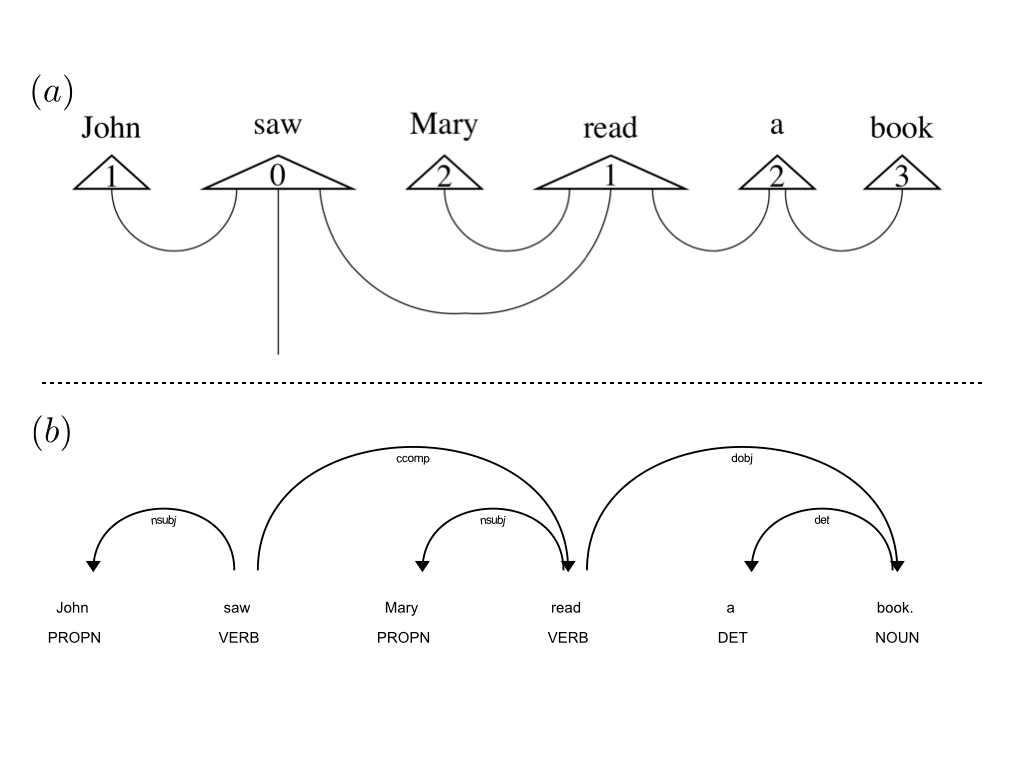
\includegraphics[width=0.85\linewidth,trim=0 20px 0 20px]{D1_1/Images/spacy_vs_CSC.png}
    \caption[DisCo model versus spaCy sentence analysis.]{Sentence parsing structure for $(a)$ the DisCo model, and $(b)$ that from the classical NLP package spaCy.}
    \label{fig:spacy_vs_disco}
\end{figure}